% **************************************************************************** %
%                                                                              %
%                                                     ::::::::  :::::::::      %
%    sec_intro.tex                                   :+:    :+: :+:    :+:     %
%                                                    +:+        +:+    +:+     %
%    By: A. Campo <andoitzcp@gmail.com>              +#+        +#++:++#+      %
%                                                    +#+        +#+            %
%    Created: 2022/11/18 22:55:54 by A. Campo        #+#    #+# #+#            %
%    Updated: 2022/11/22 06:19:19 by A. Campo         ########  ###            %
%                                                                              %
% **************************************************************************** %

\section{INTRODUCION}

El sector de la automocion,
engloba una gran variedad de industria y servicios dedicados a servirla.
Se estima que la aportacion economica total de las actividades relacionadas,
en este sector, aciende a un 11\% del PIB,
lo que la convierte en la industria manufacturera que mas ingresos aporta
despues  del 18,8\% del PIB que posee la industria agroalimentaria española
(Díaz y Montorriol Garriga, 2021).
Esta cifra puede ser contrastada
frente a la carta emitida por el presidente de la ANFAC,
adherida al informe anual,
donde se aprecian estimaciones similares.

En este sector, el vehiculo de propulsion autonoma,
es generalmente utilizado tanto por los servicios de transporte a pasajero,
como por los servicios logisticos dedicados al transporte de mercancias.
Entre los componentes que forman el vehiculo autonomo,
se encuentran las cubiertas o nematicos,
los cuales se comportan como enlace entre el vehiculo y el pavimento.
Este nexo permite una transmision eficiente
de la energia producida por el motor de combustion interna,
y a su vez, sus propiedades elasticas atenuan las irregularidades de la via.

La industria manufacturera de cubiertas,
ha mantenido un incremento sostenido en su produccion en los ultimos años,
como puede observarse en la Figura \ref{fig:1_global_prod_evo}.
El mercado de neumaticos es liderado por dos empresas: Bridgestone y Michelin
\citep{rodgers2020tire}
Las demas empresas compiten entre ellas
a un magnitud inferior a los lideres del sector,
como se aprecia en la Figura \ref{fig:1_brand_revenue}

\begin{figure}[h]
	\begin{center}
		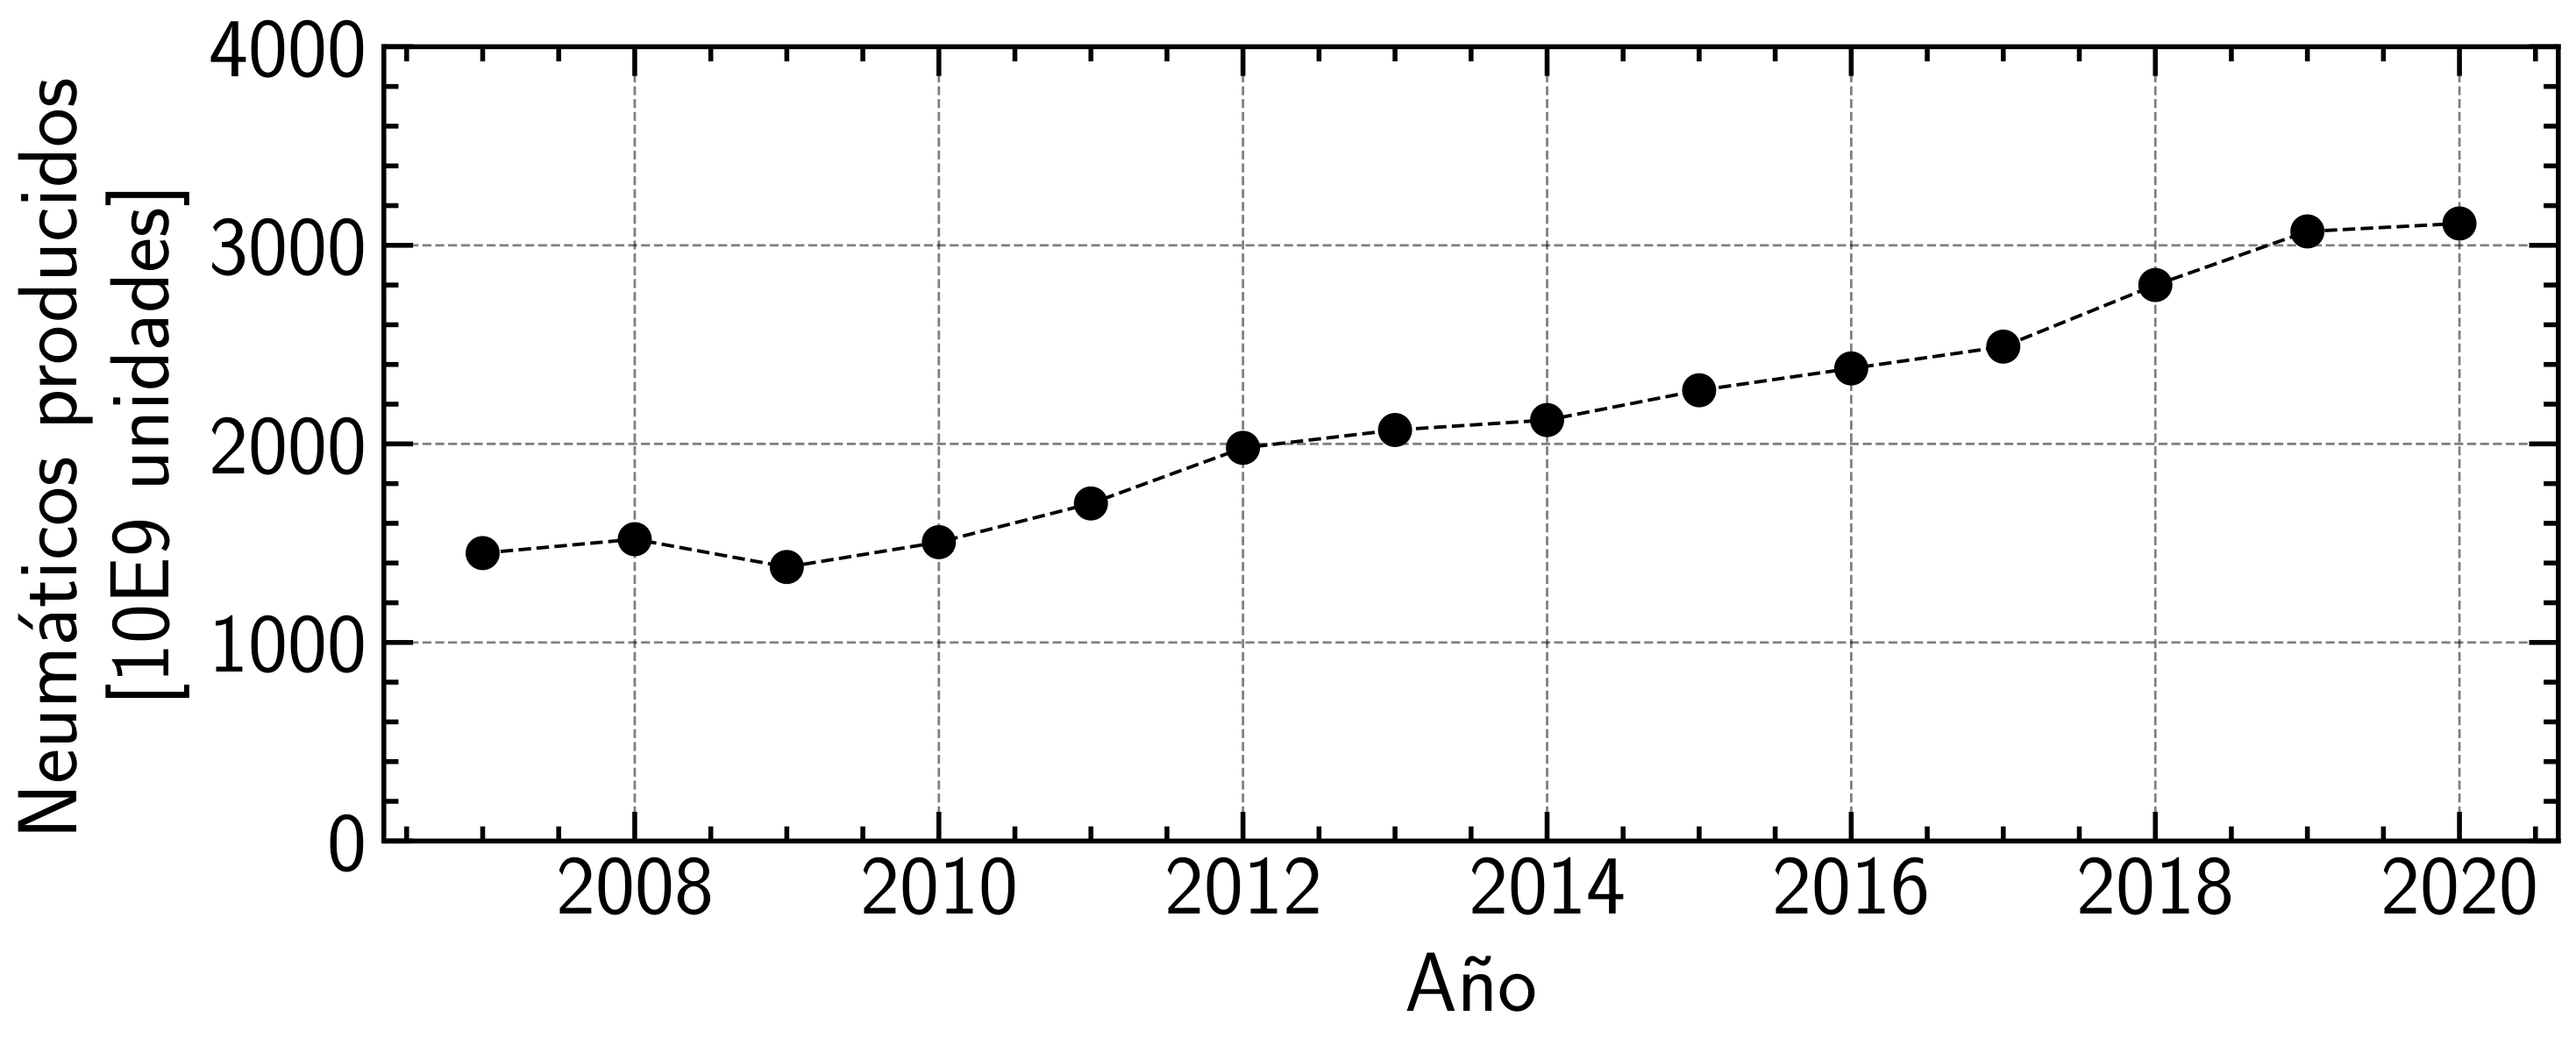
\includegraphics[width=\textwidth]{global_prod_evo.PNG}
	\end{center}
	\caption{Evolución de la producción mundial de cubiertas.}
	\label{fig:global_prod_evo}
\end{figure}

 \begin{figure}[h]
	\begin{center}
		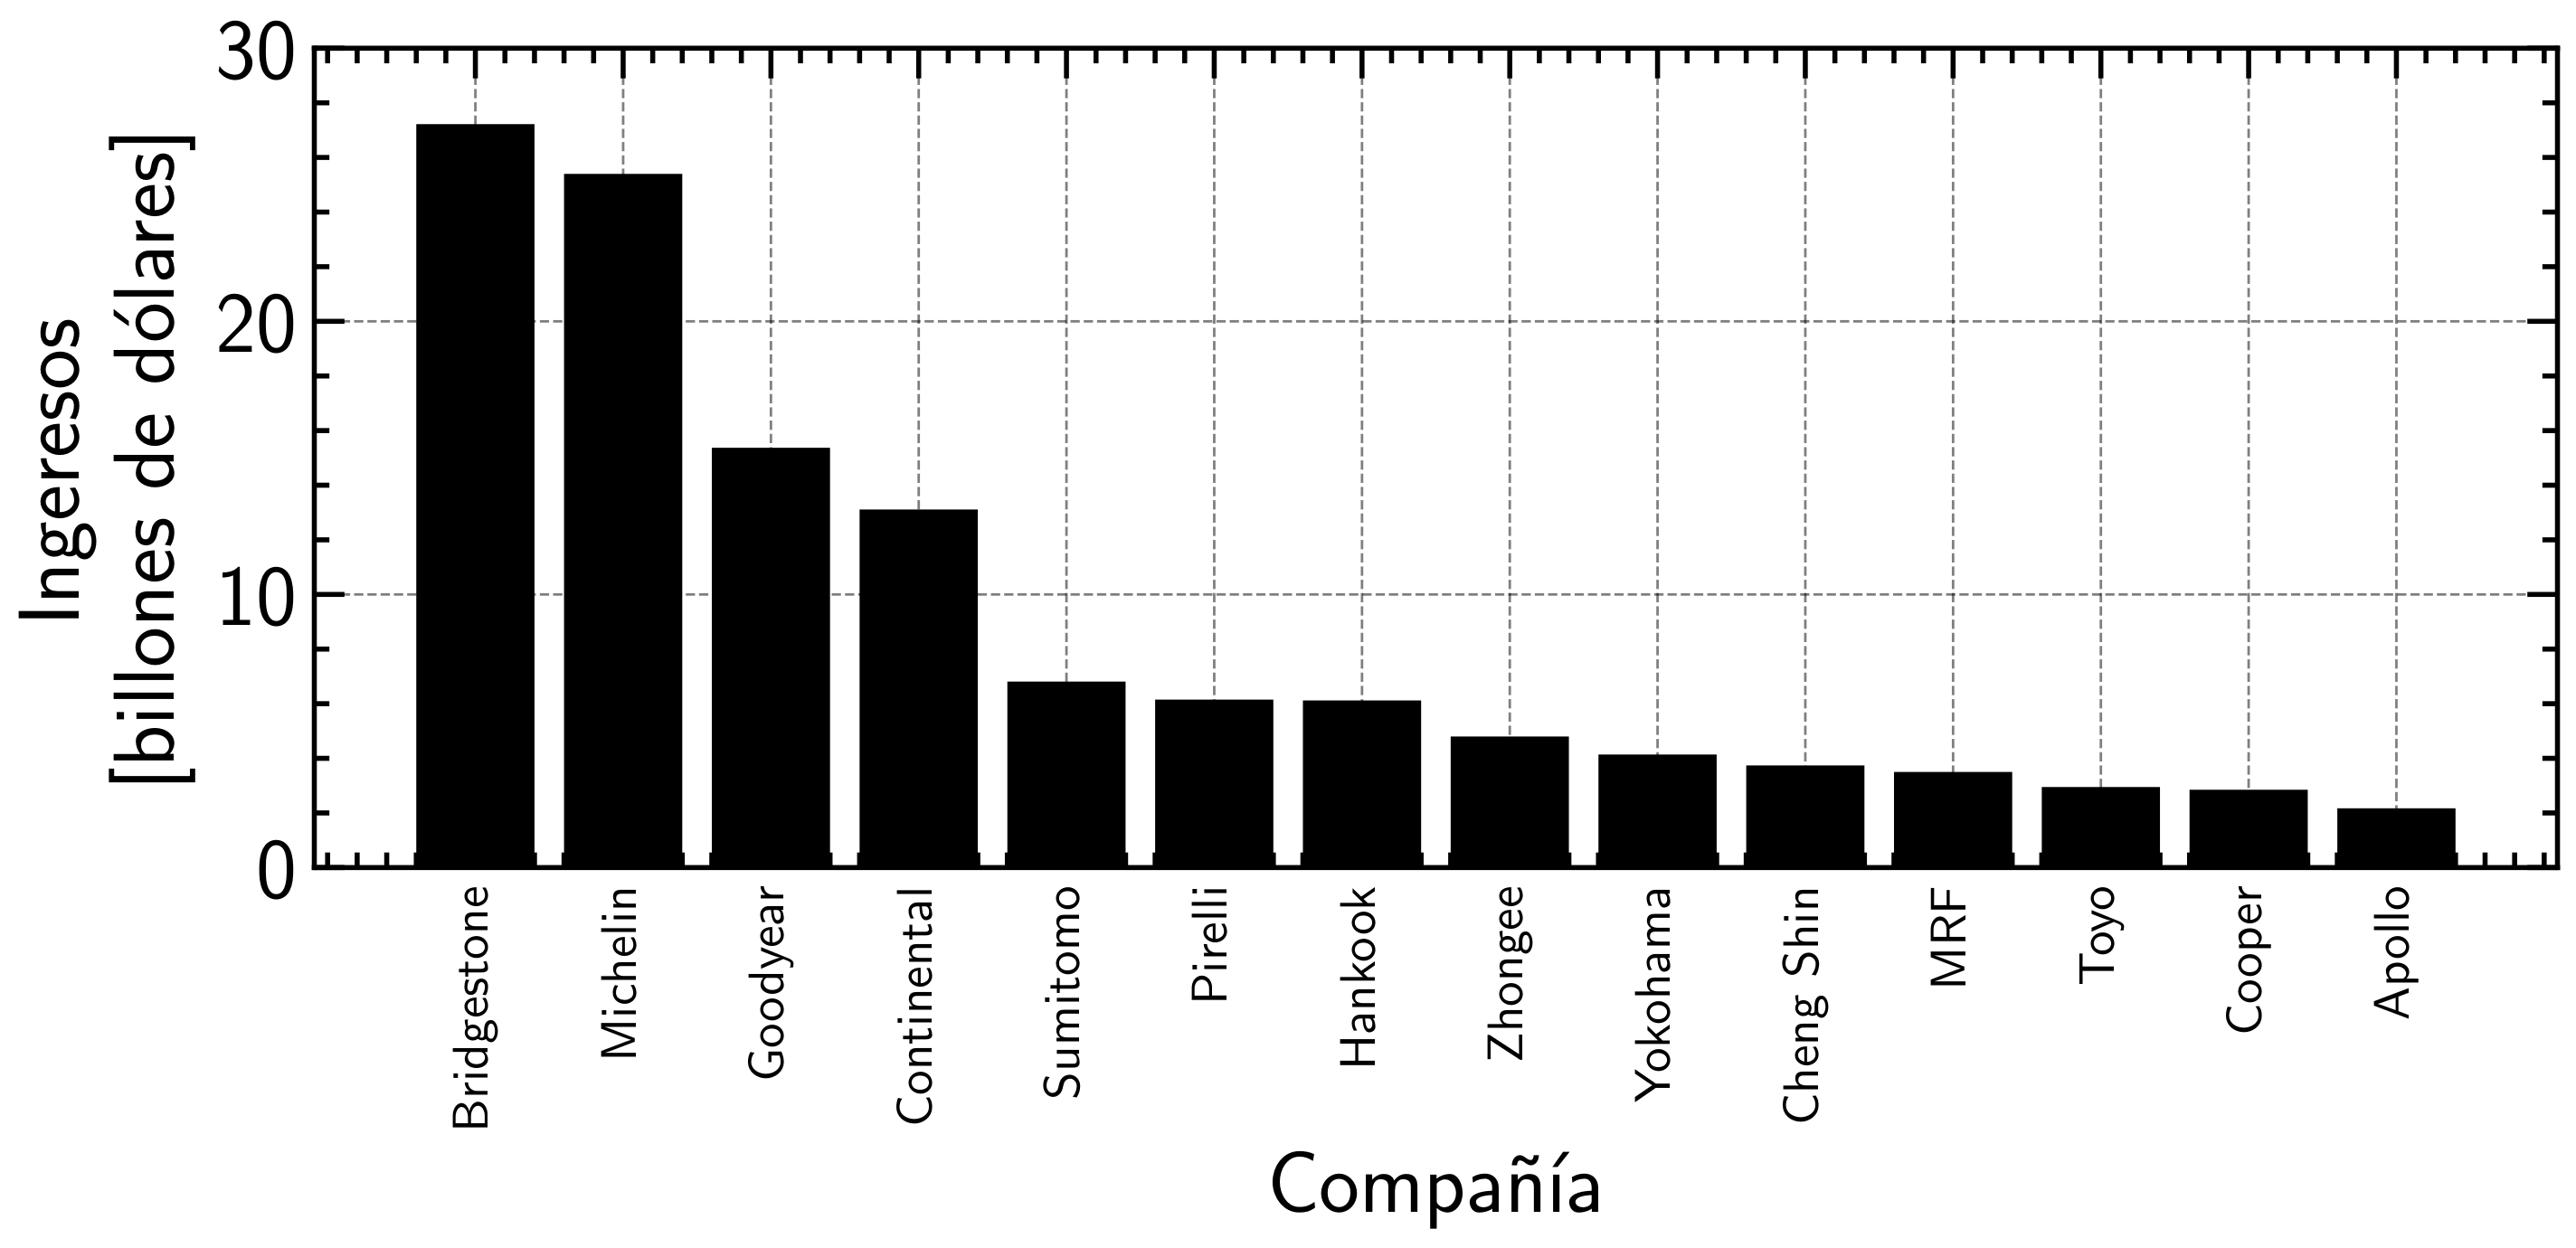
\includegraphics[width=\textwidth]{brand.revenue.PNG}
	\end{center}
	\caption{Ingresos de los fabricantes de neumáticos más relevantes en 2019.}
	\label{fig:brand_revenue}
\end{figure}

La elevada competitividad caracteristica del mercado,
sumada a la emergente comercializacion de producto asiatico,
incentiva a las establecidas multinacionales, a tomar un enfoque innovativo,
con la intencion de mantener su liderazgo \citep{chicu2020current}.
El esfuerzo invertido en innovacion,
por una parte, intenta alcanzar sus objetivos
mediante el rediseño y la mejora del producto.
Mientras que por la otra,
Trata de optimizar sus procesos y reducir desperdicios,
mediante la automatizacion y el uso inteligente de los recursos disponibles.

A la hora de implementar mejoras, ya sea a un producto o a un proceso,
la monitorizacion de los resultados y del cambio percibido se vuelve esencial.
El producto o proceso experimental debe satisfacer las expectativas del cliente,y a su vez, cumplimentar la legislacion vigente,
como los estandares de calidad y medio ambiente.
La monitorizacion de estas mejoras implica un coste elevado,
a nivel temporal y economico, ya que estas deben ser puestas a prueba.
En el caso del producto, su industrializacion,
supone reservar recursos que podrian ser destinados a la produccion regular.
Desde la materia prima utilizada
en la elaboracion de estos productos experimentales,
transitando por cada maquina ocupada para transformarlo,
hasta llegar a el laboratorio de calidad,
donde se realizan ensayos para otorgar feedback a el nuevo proceso.

El laboratorio de Calidad del Producto (LCP),
es el encargado de llevar a cabo los ensayos relevantes
para asegurar la conformidad de la produccion.
A diario se cerciora de que los neumaticos manufacturados dentro de la planta
cumpla con los estandares de calidad definidos por la compañia.
El laboratorio logra asegurar la calidad del producto,
mediante un control estadistico de las muestras
elegidas al azar por cada ganma de producto.
Paralelamente, una fraccion de los recursos disponibles,
es demandada por los proyectos de industrializacion.
Obligando al departamento a equilibrar ambas necesidades.

En un entorno con recursos limitados,
donde la demanda no cesa de incrementar,
es cuestion de tiempo que los recursos se agoten
y la capacidad de el laboratorio se vea paralizada.
Para hacer frente a esta situacion,
y poder mantener el esencial ritmo
marcado por los estandares de control de calidad e industrializacion,
debe realizarse un escalado de los recursos del LCP.
A fin de que esta expansion, de este sistema complejo,
sea realizada de la manera optima,
debe realizarse un estudio de el impacto
de las inversiones que podrian realizarse, en la capacidad del LCP.
Para realizar esta tarea,
se ha optado por diseñar una Simulacion de Eventos Discretos (DES)
que prevea los posibles futuros escenarios,
al cambiar algunas de las variables independientes de entrada.

El autor de este trabajo, se ha decantado por este metodo,
debido a la capacidad que ha demostrado
a la hora de resolver problemas de optimizacion en sistemas estocasticos.
Como menciona el autor \citep{allen2011introduction},
su versatilidad ha sido demostrada en numerosos ambitos,como
aplicaciones militares,
sistemas sanitarios,
problemas logisticos
y optimizacion de procesos de manufacturacion.

\subsection{OBJETIVOS}
El objetivo principal de este trabajo
es proveer a la planta hipotetica de cubiertas
con la informacion necesaria para la optima expaansion del LCP.
Este trabajo se limitara a analizar los distintos escenarios investigados,
ofreciendo metricas e informacion cualitativa sobre las distintas posibilidades,para finalmente decantarse por las 2 o 3 mejores opciones.

Para lograr el objetivo final se deberan completar los siguientes subobjetivos:

\begin{itemize}
	\item Modelar los procesos del LCP
		de acuerdo a los fundamentos de una DES,
		obteniendo un modelo ajustado a la realidad.
	\item Definir las variables independientes del proceso,
		que posteriomente seran usadas en la simulacion.
	\item Estimar el tiempo de ciclo de cada proceso,
		a traves de la asignacion de
		distribuciones ajustadas a cada subproceso.
	\item Definir las variables dependientes
		que otorgara el sistema a la salida.
		Estas variables, seran los indicadores o KPIs
		usados para evaluar el rendimiento del sistema.
	\item Desarrollar un programa de simulacion en el entorno de Python
		mediante el uso de la libreria Simpy.
		Dicha simulacion, sera capaz de emular
		los distintos escenaris propuestos en la metodologia.
\end{itemize}
